\section{Results}

  \subsection{Three-Tone Shading}

      The results of the three tone shading can be seen in Figures
      \ref{three-tone-1} and \ref{three-tone-2}.  Looking at these the technique
      is definitely working effectively.  Likely the biggest flaw is the lack of
      crease lines to identify areas of sharp model curves.  The silhouette
      edges have been drawn showing where parts of the model overlap other
      parts, most noticeable around the body-leg joins and the edge of the horse
      head.  These help a lot in identify the depth of the model, but adding in
      crease lines along areas such as the edge of the leg muscles on the
      horse's body and down the camel's body between the humps would greatly
      enhance the differentiability of these attributes.

    \begin{figure}
      \centering
      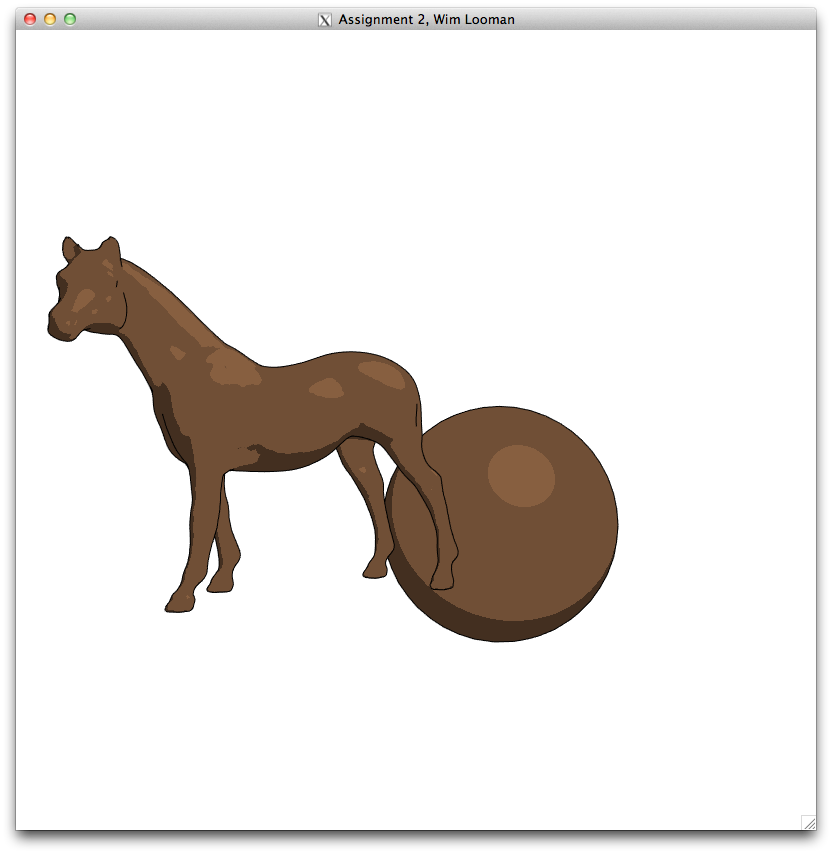
\includegraphics[width=0.45\textwidth]{images/three-tone-1}
      \caption{Three tone-shading of a horse.}
      \label{three-tone-1}
    \end{figure}

    \begin{figure}
      \centering
      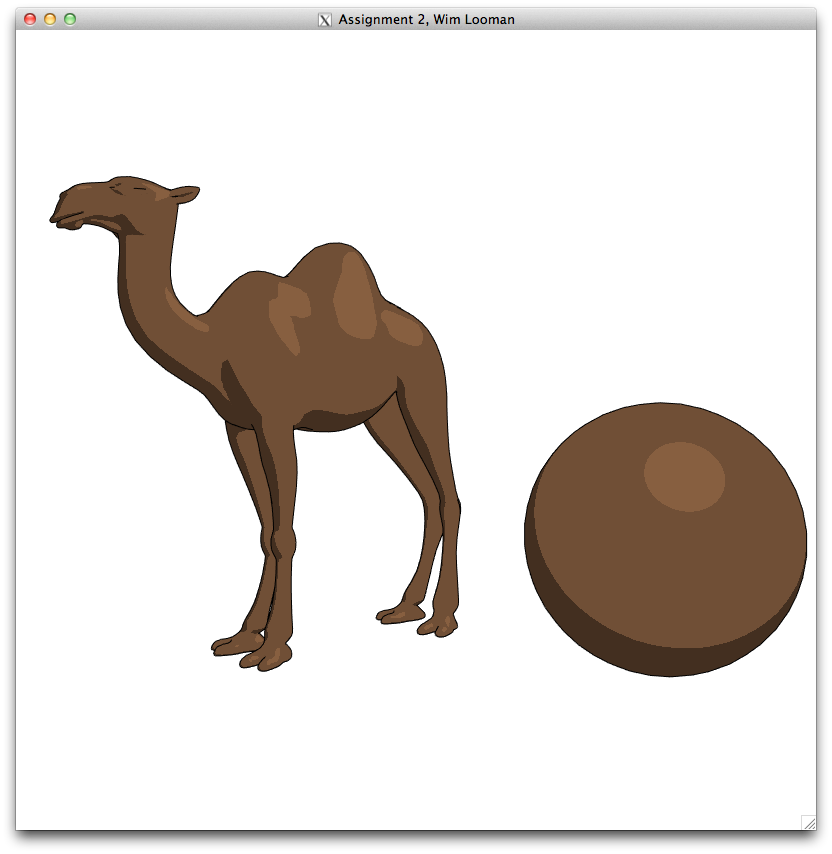
\includegraphics[width=0.45\textwidth]{images/three-tone-2}
      \caption{Three tone-shading of a camel.}
      \label{three-tone-2}
    \end{figure}

  \subsection{Pencil Shading}

      Figures \ref{pencil1}, \ref{pencil2}, \ref{pencil3} and \ref{pencil4} show
      the pencil shading result on a horse and camel model, along with close ups
      of a part of each.

      Close up the pencil shading doesn't look too bad, the largest flaw is
      probably the fact that the lines don't meet up very well.  At distance the
      lines sort of become a mess however, this is mainly because of the lack of
      mipmapping.  If the texture was mipmapped then the view further out would
      be greatly enhanced.  However the very simple single pixel line texture
      used is not conducive to automatic mipmapping.

      So really the greatest enhancement would be provided by having a better
      pencil texture either generated or pre-drawn and loaded at run-time.  For
      example the stroke generation by Mario Costa Sousa and John W. Buchanan
      \cite{graphite} shown in Figure \ref{graphite} looks much better, using
      the method they propose to generate the textures would likely make the
      pencil shading a lot more lifelike.

    \begin{figure}
      \centering
      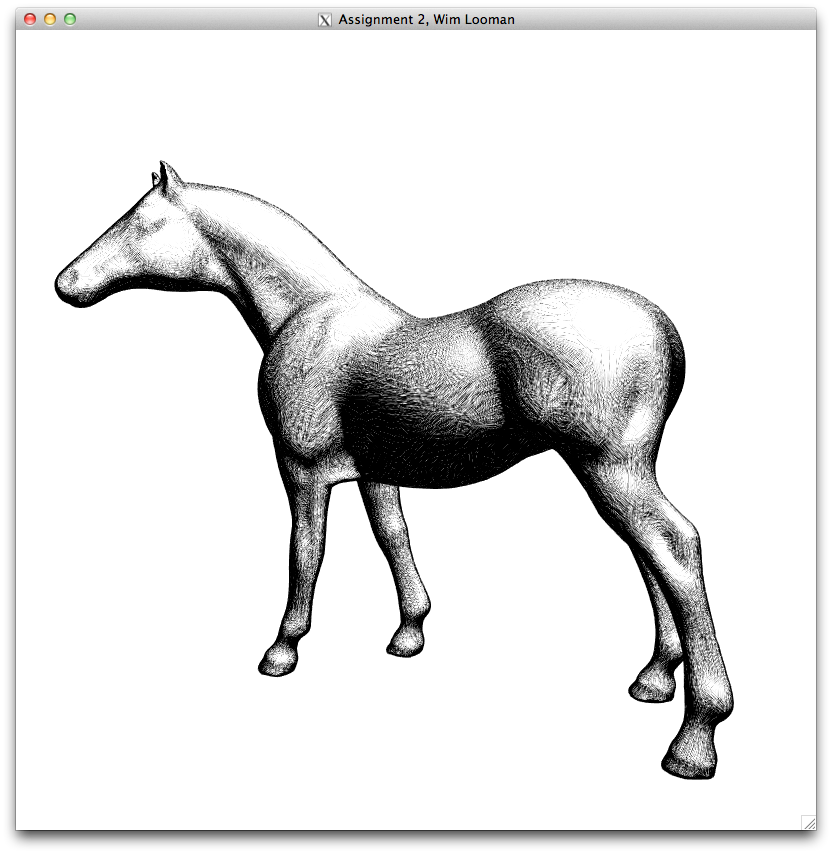
\includegraphics[width=0.45\textwidth]{images/pencil-1}
      \caption{Pencil shading of horse model.}
      \label{pencil1}
    \end{figure}

    \begin{figure}
      \centering
      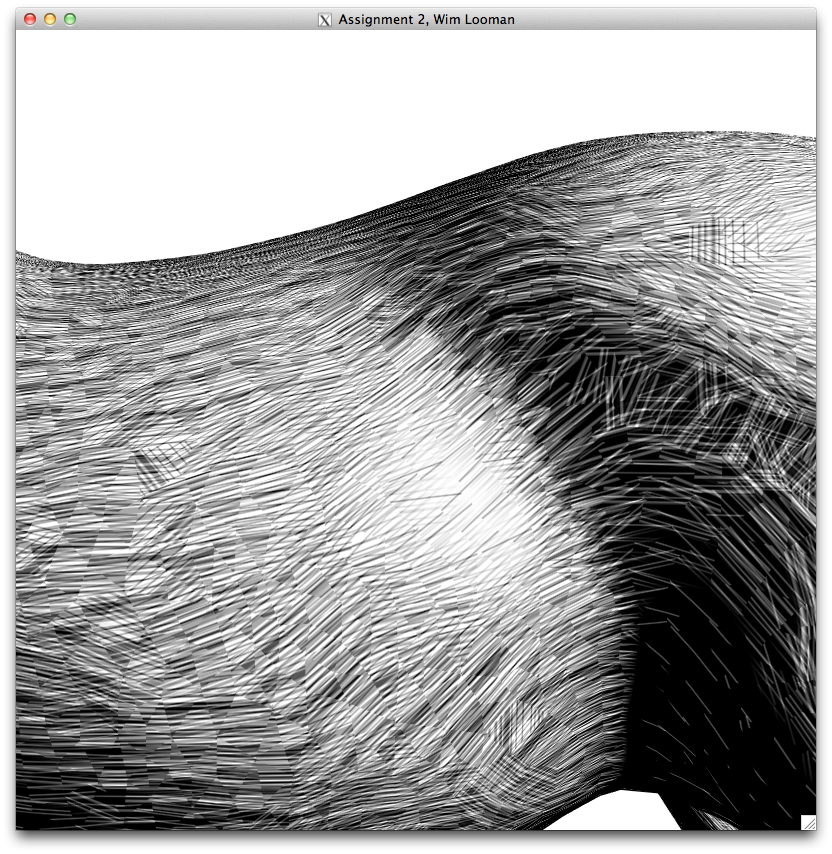
\includegraphics[width=0.45\textwidth]{images/pencil-2}
      \caption{Close up of horse model.}
      \label{pencil2}
    \end{figure}

    \begin{figure}
      \centering
      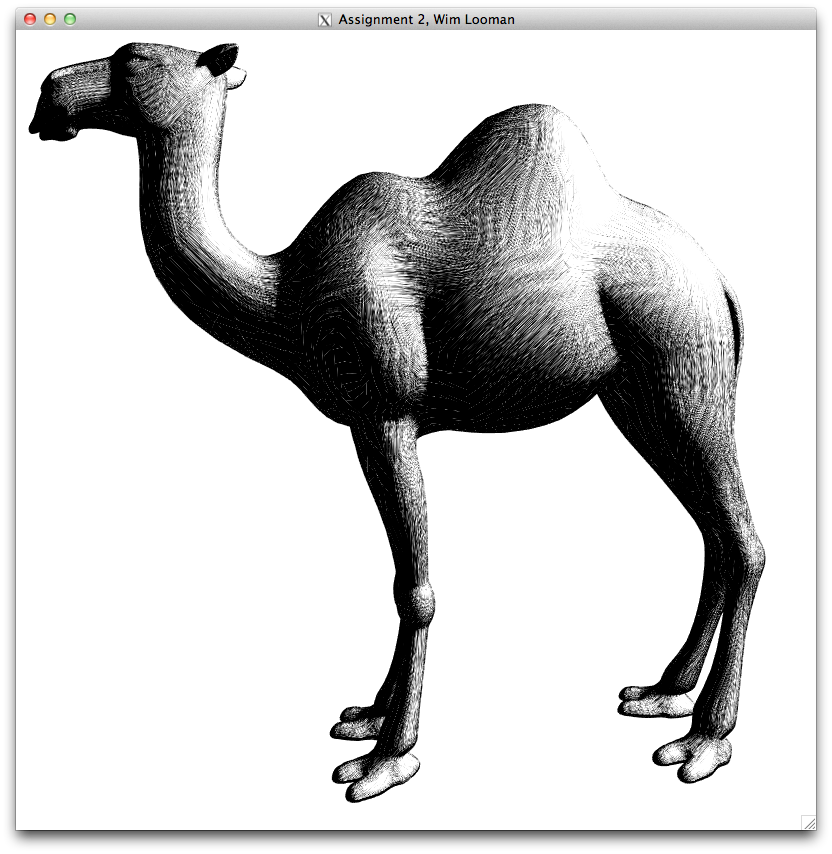
\includegraphics[width=0.45\textwidth]{images/pencil-3}
      \caption{Pencil shading of camel model.}
      \label{pencil3}
    \end{figure}

    \begin{figure}
      \centering
      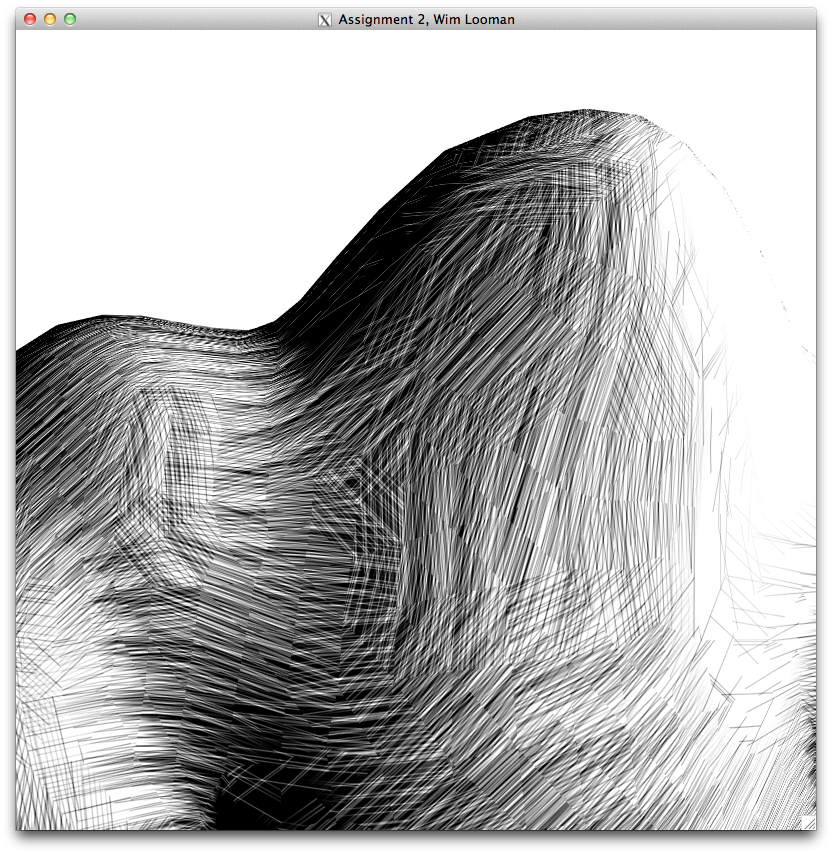
\includegraphics[width=0.45\textwidth]{images/pencil-4}
      \caption{Close up of camel model.}
      \label{pencil4}
    \end{figure}

